\section{System Overview} \label{sec.system}

\begin{figure*}[htb]
\centering
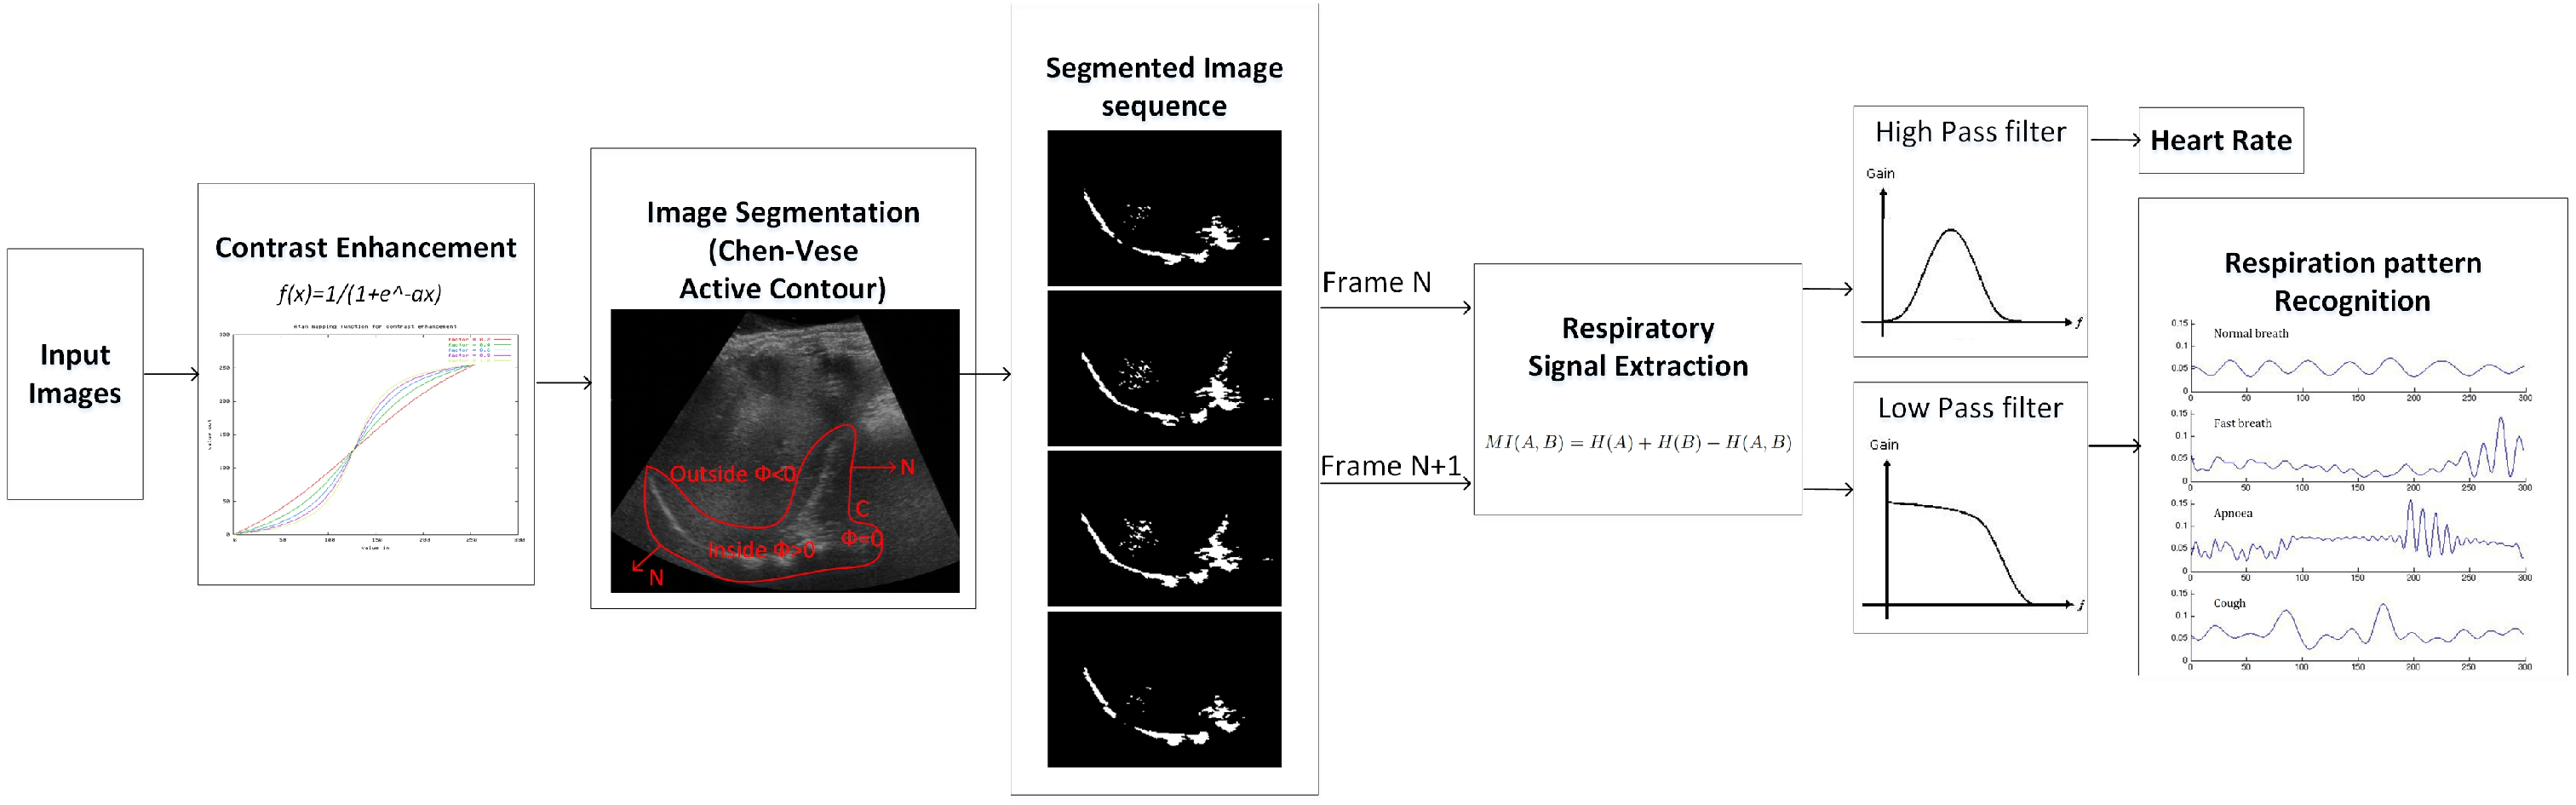
\includegraphics[width=1\textwidth]{flowchart.pdf}
\caption{Image analysis flowchart}
\label{fig.flow}
\end{figure*}
In this section, the system design of asthma pattern identification is discussed. It consists of six parts: a USB ultrasound imaging probe, ROI Identification, 2D Image Sequence to 1D Time Series, heartbeat removal, respiratory pattern recognition for asthma, and visualization, as shown in Figure~\ref{fig.System}.

First of all, ultrasound probe collects ultrasound image sequences around liver and diaphragm locations. Then these images are transmitted via USB to a computer. In this paper, the goal is to monitor the movement of diaphragm to extract respiratory signal, so system identifies and segments the diaphragm area in the image sequence, and then computes 1D time-series signal drawn by mutual information (MI) which reflects relation among consecutive ultrasound image sequence. The original 1D waveform contains respiratory signal and unwanted interference, such as cardiac signal. Therefore, a low-pass filter is used to get rid of interference and preserve low respiratory frequency. Next, the computed 1D signal is compared to four templates: normal breath, fast breath, apnoea, and coughing. In the end, ultrasound video, original signal, purified signal, and respiration rate are displayed on a designed Matlab user interface.
\subsection{Ultrasound Sensor System}
In experiments, an ultrasound probe from Interson company is used, which is a USB ultrasound probe system. Detailed technical specifications are listed in Table~\ref{tab.Spec}.
\begin{table}
\newcommand{\tabincell}[2]{\begin{tabular}{@{}#1@{}}#2\end{tabular}}
 \centering
 \begin{tabular}{|c|c|}\hline
Depth Range & \tabincell{c}{2-15 cm } \\\hline
Pulse Frequency & \tabincell{c}{3.5-5MHz} \\\hline
Frame Rate & \tabincell{c}{12 fps } \\\hline
Scan Angle & \tabincell{c}{60 degrees } \\\hline
Image Format & \tabincell{c}{Jpeg } \\\hline
Image Size & \tabincell{c}{$1024\times600$} \\\hline
Gray Scale & \tabincell{c}{256 shades } \\\hline
Scanning Mode & \tabincell{c}{B-mode } \\\hline
\end{tabular}
\vspace{0.3 cm}
\caption{Technical specifications of Interson ultrasound imaging probe}
\label{tab.Spec}
\end{table}
This transducer converts ultrasound waves to electrical signal and perform B-mode scanning to generate ultrasound images. Images are transmitted to a computer via USB. Direct streaming of B-mode ultrasound images is used over this system. As the ultrasound waves penetrate body tissues of different acoustic impedances, some are reflected back to the transducer (echo signals) and some continue to penetrate deeper. The echo signals returned from many sequential coplanar pulses are processed and combined to generate an image. The pulse frequency of this probe is 3.5 to 5 MHz and the largest scan depth is about 15 cm. It can detect the movement of organs and tissues in our body, such as a liver, kidney, lung, and diaphragm. The sample frequency is 12 frames per second which is much higher than the breathing frequency. The collected data are high quality JPEG images with 256 shades of gray scale. Image size is $1024\times600$ pixels.

\subsection{Image Analysis}
Collected images are processed to extract respiratory signals, and use these signals to compute the breathing rate and evaluate the respiratory pattern. Image analysis contains segmentation of ROI, 1D respiratory signal extraction with MI method, and filter. Finally, the purified respiratory signal is compared with the stored templates to classify pattern of asthma. The image analysis flowchart is shown in Figure~\ref{fig.flow}.

\textbf{4.2.1 Chan-Vese active contour}

 This system implements the Chan-Vese active contour algorithm~\cite{Chan:2001} to find ROI. The basic idea of this model is that starting with a curve around the objects, the curve extends or shrinks toward its interior normal, and stops when touch the boundary of the objects. Given an image $u_0$, the goal is to look for the best approximation $u$ of $u_0$ by minimizing an energy function $F(c_1, c_2, C)$. $u$ is the segmented result and it takes two values:
\begin{equation}
u=
\begin{cases}
average(u_0),  &\mbox{ inside C}\\
average(u_0),  &\mbox{ outside C}\\
\end{cases}
\end{equation}

Notations are illustrated in Figure~\ref{fig.curve}. The energy function $F(c_1, c_2, C)$ is defined by\\
\begin{align*}
F(c_1, c_2, C) =&\mu \int_{\Omega}\delta(\phi (x, y))|\bigtriangledown\phi(x, y)|{d}x{d}y\\
                    &+\nu \int_{\Omega}H(\phi (x, y)){d}x{d}y\\
                    &+\lambda _1\int_{\Omega}|u_0(x, y)-c_1|^2H(\phi (x, y)){d}x {d}y\\
                    &+\lambda _2\int_{\Omega}\mid u_0(x, y)-c_2\mid ^2\\
                    &(1-H(\phi (x, y))){d}x{d}y\\
\end{align*}
where $C$ is an arbitrary variable curve, and constants $c_1$, $c_2$, depending on C, are averages of $u_0$ inside $C$ and respectively outside $C$. $\mu \geq0$, $\nu \geq0$, $\lambda _1$, $\lambda _>0$ are fixed parameters and function $H$ is the Heaviside function, defined by:
\begin{equation}
H(z)=
\begin{cases}
1,  &\mbox{ if $z \geq 0$}\\
0,  &\mbox{ if $z \leq 0$}\\
\end{cases}
\end{equation}
In this equation, the first item is the length of curve and the second item is the area of the region inside. They are the regularizing items.
Primary steps of the algorithm are shown in Algorithm 1.
\begin{algorithm}
\caption{Chan-Vese active contour algorithm}
\begin{algorithmic}
%\STATE
\STATE /* Initialization */
\STATE Step 1: $\phi^0\leftarrow\phi _0, n\leftarrow0$.
%\STATE
\STATE /* Iteration */
\STATE Step 2: Compute $c_1(\phi^n)$ and $c_2(\phi^n)$.
\STATE Step 3: Solve the PDE in $\phi$ to obtain $\phi^n+1$.
\STATE Step 4: Reinitialize $\phi$ locally to the signed distance function to the curve (this step is optional).
\STATE Step 5: If the solution is stationary, stop,
\STATE \qquad \qquad otherwise go to Step 2.
\end{algorithmic}
\end{algorithm}

\textbf{4.2.2 Breathing signal extraction}
Mutual information (MI) is computed as the 1D signal. MI measures statistical dependence of two images and is defined by
\begin{align*}
MI(A,B) &=H(A)+H(B)-H(A, B)\\
            &=\sum\limits_{ab} p(a, b)log\dfrac{p(a, b)}{p(a)p(b)}\\
\end{align*}
Here, $A$ and $B$ are ROI from two consecutive image frames. $H(A)$, $H(B)$, and $H(A, B)$ are the entropies of $A$ and $B$, and their joint entropy respectively. $p(a, b)$, $p(a)$ and $p(b)$ are the joint probability distribution of $a$ and $b$, and their individual probability distributions, where $a$ and $b$ are the pixel values in $A$ and $B$.
An image at the end of inspiration is selected as a reference image. MI between this frame and all other segmented image frames were computed. Large MI value occurs when diaphragm is close to the reference frame, i.e. the end of inspirations. On the contrary, small MI value occurs when the diaphragm motion is far away from the reference. Thus 1D signal's magnitude and phrase are related to respiration.

\begin{figure}[h!]
\centering
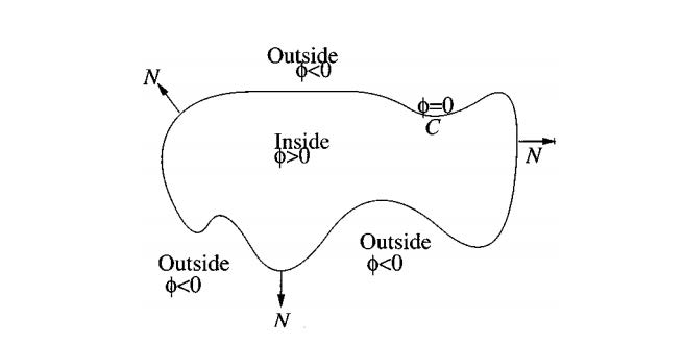
\includegraphics[width=0.36\textwidth]{curve.pdf}
\caption{Curve \textbf{$C=(x, y): \phi(x, y)=$} propagation in normal direction}
\label{fig.curve}
\end{figure}


\textbf{4.2.3 Heartbeat removal}
During ultrasound images recording, the two most common sources of diaphragm motion are respiratory and cardiac motions. For the reason that asthma attack detection is only based on respiration, the cardiac signals are interference. According to Hari et al.~\cite{Hari:2009}, the cardiac signal is approximately centered at 1Hz. The time of one respiration cycle is about three seconds recorded by chronograph and the frequency of respiratory signal is around 0.3 Hz. Then the cardiac signal the respiratory signal are separated with a low pass filter.

\textbf{4.2.4 Asthma pattern templates creation}
Before asthma attack, patients usually feel some symptoms, like fast breathing, short of breath, and coughing. These symptoms will induce the change of the respiratory pattern. In this paper, four typical respiratory waveforms are used as templates, one regular template and three irregular templates: normal breath, fast breath, apnoea and cough. Fast breath is due to short of breath. Subject needs to increase breathing frequency to overcome the difficult breathing caused by narrow airways. If airways are more and more narrow, subject has the potential to get apnoea and stop breathing. Coughing also changes the breathing status. Building templates of irregular patterns is very useful for detecting asthma attack. Respiratory signal is partitioned into time segments and compare each segment with templates. Then it is efficient to identify which irregular activities happens and their occurring order.

\subsection{Visualization}
For convenience, system has a Matlab user interface to display the respiratory signal and respiration rate, as shown in Figure~\ref{fig.GUI}. Designed system could detect subject's real-time respiration status based on the movement of the diagram. The user interface contains three parts, the left part displays the ultrasound video obtained by the probe and the 1D respiratory signal. The 'operation' panel consists of four push buttons: Start, End, Filtered, and Original. When 'Filtered' button is clicked, it shows the purified respiratory signals without heartbeat interference. When click 'Original' button, it shows the mixture of heartbeats and breathing signals. 'Respiration rate' panel shows the number of respiration cycles per minute and it renews every minute.

\begin{figure}[h!]
\centering
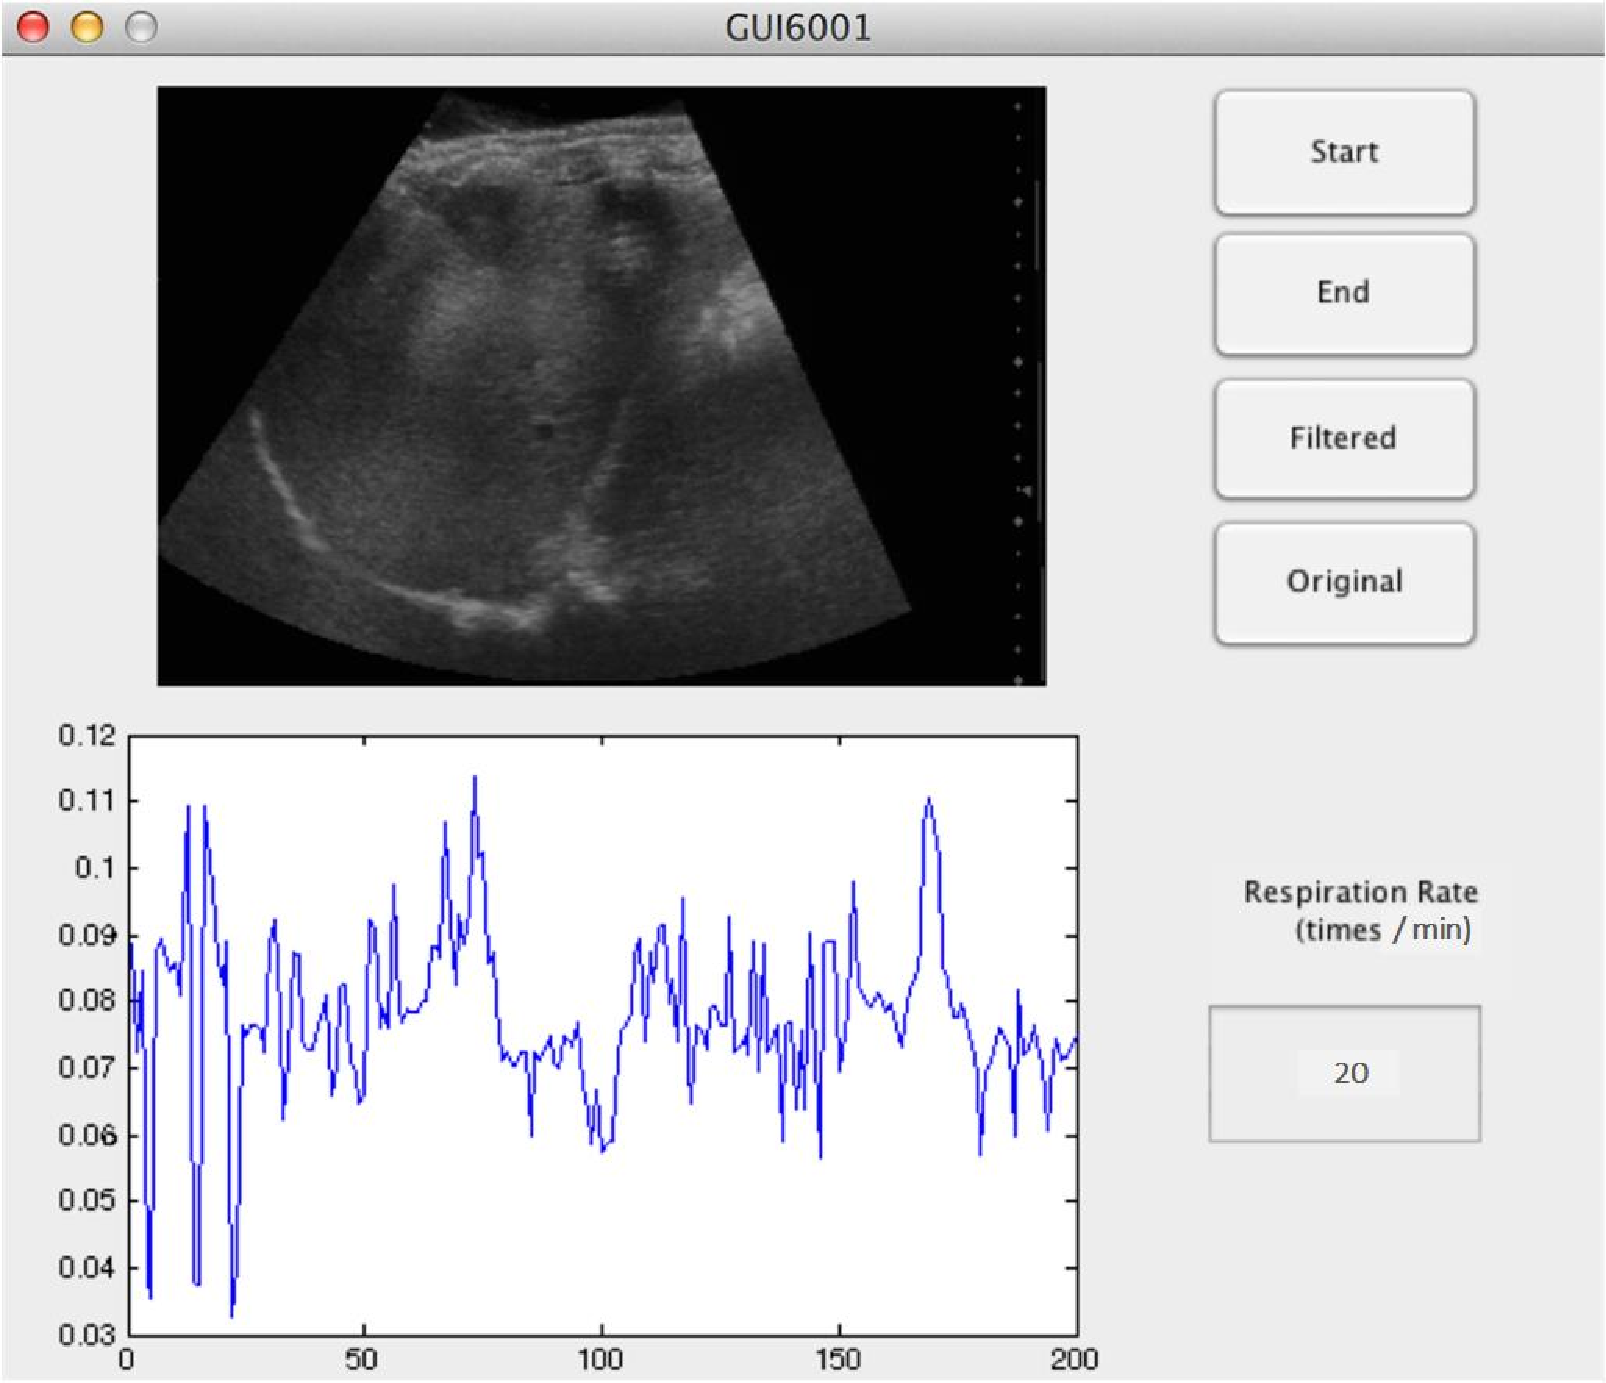
\includegraphics[width=0.36\textwidth]{MatlaGUI.pdf}
\caption{User interface design}
\label{fig.GUI}
\end{figure}
